\section{Strain Gauge Measurement}

\subsection{Electrical}
The Texas Instruments ADS1148 (Q1 Automotive) $\Delta\Sigma$ (Delta Sigma) Analog-Digital-Converters are used within HERMESS for the measurements of the strain gauge rosettes.

As shown in figure \ref{fig:wheatstone}, one wheatstone bridge for each rosette is used for temperature compensation of the sensors themselves and increase of measurement accuracy. They will be excited with the on-board standard voltage of $3.3V$. Resistors with a resistance of $1k\Omega$ form the counterpart of the halfbridge configuration. The ADC will then measure the fully differential voltage across the measurement bridge. It is important to note, that the wire resistances for the STAMP connections are not compensated and therefore should be kept minimal and equal for the both non-bridge-wires.

\begin{figure}[htb]
	\centering
	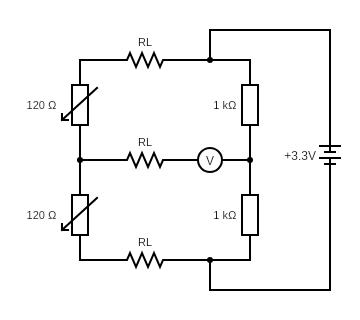
\includegraphics{ADC/wheatstone.png}
	\caption{Wheatstone bridge used for strain gauge rosettes}
	\label{fig:wheatstone}
\end{figure}

The ADC uses for analog and digital voltage supply the standard 3.3 volts.

\begin{equation}
\begin{split}
DVDD = AVDD &= 3.3V \\
DVSS = AVSS &= 0V
\end{split}
\end{equation}

Assuming a maximal differential voltage of $V\textsubscript{IN, max} = 200mV$ on the bridge, which was excited with $3.3V$, fulfills all electrical requirements for the ADCs input range.

\begin{equation}
\begin{split}
V\textsubscript{AINX, max} = \frac{3.3V}{2} + \frac{200mV}{2} = 1.25V\\
V\textsubscript{AINX, min} = \frac{3.3V}{2} - \frac{200mV}{2} = 1.05V\\\\
(\mbox{AVSS} - 100mV) < V\textsubscript{AINX} < (\mbox{AVDD} + 100mV)
\end{split}
\end{equation}

The gain of the Programmable Gain Amplifier (PGA) can be set to values between in the range of $2^0$ and $2^7$ with increments of exponents with the base 2. The internal reference voltage of $V\textsubscript{REF} = 2.048V$ will be used. The differential full-scale input voltage range (FSR) of the PGA is defined by the gain setting and the reference voltage used. This leads us to a gain setting of 16.

\begin{equation}
\begin{split}
\mbox{FSR} &= V\textsubscript{REF} / \mbox{Gain}\\
200mV &\geq 2.048V / \mbox{Gain} \\
\mbox{Gain} &\geq 10.24
\end{split}
\end{equation}

Given the Common-Mode Voltage $V\textsubscript{CM} = \frac{3.3V}{2} = 1.15V$, the electrical requirements for the ADC-internal PGA are also met.

\begin{equation}
\begin{split}
V\textsubscript{CM (MIN)} &\geq \mbox{AVSS} + 100mV + \frac{1}{2} \mbox{Gain} \times V\textsubscript{IN, max} \\
V\textsubscript{CM (MAX)} &\leq \mbox{AVDD} - 100mV - \frac{1}{2} \mbox{Gain} \times V\textsubscript{IN, max}
\end{split}
\end{equation}

As shown in attachment !!!, a simple analog RC lowpass filter is used for $3dB$ attenuation at approximately 2kHz.


\subsection{Software}
After the Device was powered up, it is held in a reset state for $2^{16}$ clock cycles. During that time, it resets all registers and cannot be controlled via SPI. After that time, it needs additional $0.6ms$ to enable communication and filtering. The Reset can be triggered by pulling the RESET-pin low or via an SPI command.

The device will continuously convert and not enter sleep mode, when the start pin is constantly pulled high. This also enables the configuration of the registers. For our experiment, we need to signal the exact timings of the conversion, thus the SYNC command has to be sent to all devices at the same time. This will stop the current conversion and immediately begin a new one. Once converted, the DRDY pin is being pulled low by the ADC.

The SCLK period must not exceed 520ns, and the time between the beginning of writing a register byte data and the beginning of a subsequent register byte data must not exceed 4.2us. Between writing to multiple registers, wait at least 64 clock cycles.

Whenever a write operation to a configuration register occurs, the digital filter is being reset. The offset-calibration enables the setting of the exactly measured common-mode voltage, which will then be used as a 0-reference. For that the SYSOCAL (for measuring bridge) and SELFOCAL (for ADS) commands are sent in that order. Because the ADC internally uses 24 bit resolution, it can also apply a logical gain to the output value. For that, during testing the maximum expected load will be applied to the system and the SYSGCAL command for the ADC with the maximum force attached triggered. The resulting calibration value from the full-scale calibration register will be read out and manually reapplied, every time the system starts up again. Every calibration takes 8.07ms.

These registers are manually set by software: SYS0 (Offset: 0x03; Value: 0x4F) MUX1 (offset = 0x02; Value: 0x30).
